\section{Meilenstein 3: Entities, Components, Systems}\label{sec:meilenstein_3}

Mit dem für Meilenstein 3 geplanten Funktionsumfang standen die Umsetzung der Spielphysik und der Feuermechaniken im Fokus.

Die Anforderungen an Physik- und Waffensysteme machten jedoch schnell deutlich, dass ein klassisch objektorientierter Entwurf zu unerwünscht tiefen Vererbungshierarchien führen würde.
Im Hinblick auf die angestrebte Performance erschienen die damit verbundenen Laufzeitkosten, insbesondere virtuelle Funktionsaufrufe und \textit{VTable-Lookups}~\cite[161--164]{Gre19}, mit dem Wunsch nach einer effizienten Implementierung kaum vereinbar.\footnote{
    Wir verwenden hier explizit den Begriff ``Wunsch``, da die Anforderungen an die Performance im Prototypen-Dokument nicht ausdrücklich formuliert wurden.
}\\

Ohnehin befand sich das Projekt an dieser Stelle durch die Programmierung der Engine-nahen Systeme an einem Scheideweg: 
Die konsequente Fortführung des objektorientierten Ansatzes würde ein späteres Umstellen auf ein anderes Paradigma mit hohem Aufwand verbinden; der populäre datenorientierte Ansatz~\cite{Bay22} würde zunächst Einarbeitung erfordern und die praktische Implementierung verzögern.\\

Zwar war die in~\ref{lst:gameobject_v1} auszugsweise dargestellte API für einen einfachen Prototypen, der nur geringe Anforderungen (wie die Repräsentation lokaler Transformationen) erfüllen musste, durchaus handhabbar. 
Für die Umsetzung komplexerer Logiken wie der Feuermechanik hätten diese jedoch entweder in die Basisklasse integriert werden müssen - was zu \textit{Dead Code} bei Objekten geführt hätte, die diese Funktionalität nicht benötigen\footnote{wie etwa die geplanten Gegnertypen, die dem Originalspiel entsprechend keine Waffen führen sollen} - oder eine Spezialisierung hätte erfolgen müssen. 
Auch hier war zunächst unklar, wie in einem gewohnten OOP-Ansatz ein vernünftiger Schnitt zwischen Basisklasse und Spezialisierung hätte aussehen können.

Rückblickend lässt sich sagen, dass der praxisnahe Ansatz, zunächst nach den im Prototypen-Dokument eher vage formulierten Vorgaben zu entwickeln, mit der zu diesem Zeitpunkt noch begrenzten fachlichen Erfahrung der Entwickler kollidierte: Eine frühere Auseinandersetzung mit den fachlichen Anforderungen sowie eine Rücksprache mit der Projektbetreuung über Tragweite und architektonische Auswirkungen hätten spätere konzeptionelle Probleme bei der Trennung von Verantwortlichkeiten vermeiden können.


\begin{lstlisting}[style=c++style,
    caption={
Auszug aus dem Interface des \texttt{GameObject} (Stand Meilenstein 2). Die gleichzeitige Verwendung einer spielweltbasierten \texttt{position} und der \texttt{translation} aus dem \textit{SceneGraph} weist bereits auf eine doppelte Zustandsrepräsentation hin. Die inkonsequente Trennung sorgte in späteren Meilensteinen für Synchronisations- und Zuständigkeitskonflikte beim Hinzufügen weiterer transformationsbasierter Systeme.
},
    label=lst:gameobject_v1]
    /**
     * @brief Pointer to the SceneNode's transform component.
     */
   Transform* transform_;

    /** @brief
     * The current position-vector in local coordinates (model space).
     */
    vec3f position_{};

    /**
     * @brief Applies a scaling transformation.
     */
    GameObject& setScale(const vec3f& scale) noexcept;

    /**
     * @brief Applies a rotation transformation.
     */
    GameObject& setRotation(const mat4f& rotation) noexcept;
\end{lstlisting}

Um den Aufwand zu reduzieren und sich im Sinne des \textit{Tracer Bullet Development}~\cite[50--55]{TH20} schrittweise den Anforderungen zu nähern, wurde entschieden, die Physik- und Transformationskomponenten aus dem \texttt{GameObject} zu extrahieren.
Dieses wurde fortan, dem bereits zitierten Prinzip \textit{composition over inheritance} folgend, als reiner Komponenten-Container aufgefasst, und markierte den ersten (unbewussten) Schritt in Richtung eines datenorientierten Ansatzes.
Dass die Terminologie zu diesem Zeitpunkt zwar an ECS angelehnt ist, \textit{helios} mit Meilenstein 3 aber kein „echtes“ ECS umsetzt, wird deutlich, wenn man die Datenhaltung der für die Spielmechanik relevanten Objekte betrachtet (siehe Abbildung~\ref{fig:gameobject_uml}): Die Tatsache, dass es eine besitzende, konkret als Klasse modellierte Entität gibt (\texttt{GameObject}) und zugehörige Komponenten in nicht zusammenhängenden Speicherbereichen verwaltet werden, bricht mit dem ECS-Paradigma.
Weitere ECS-Antipatterns, die sich in der Umsetzung zeigen, sind:

\begin{itemize}
\itemsep0.5em
\item Identifizierung aller Objekte über eine \texttt{GUID}, wobei der Zugriff über die \texttt{GameWorld} hash-basiert mittels \texttt{std::unordered\_map} erfolgt.
\item Dynamisches Hinzufügen und Entfernen von Komponenten über einen \texttt{std::vector<std::unique\_ptr<Component>>}, die jedes \texttt{GamObject} besitzt.
\item Eine \texttt{GameObject::update()}-Methode zur zusätzlichen, individuellen Aktualisierung der Objekte pro Frame, wodurch eine Orchestrierung durch übergeordnete Systeme erschwert wird:
    Die Redundanz der \texttt{update()}-Methoden und die damit verbundene Dopplung der Verantwortlichkeiten sollte außerdem als \textit{Code Smell} betrachtet werden.~\cite[76]{Fow99}
\end{itemize}

Insgesamt entspricht die Umsetzung zu diesem Zeitpunkt einem ``Compound Object``~\cite[S. 88]{Fab18}, wie es ähnlich in Unity zu finden ist~\cite{UnityGameObject}; weitere Ausführungen zum \textbf{umgesetzten} ECS-Design folgen in Abschnitt~\ref{ch:ecs}.


\subsection{Steuerung des Verhaltens über Systeme}


Physik und Feuermechaniken werden als eigenständige Systeme betrachtet, die in der \textit{GameLoop} - die zu diesem Zeitpunkt noch als einfache \texttt{while}-Schleife ohne eigene Logik implementiert war - über einen zentralen Aufruf von \texttt{GameWorld::update(float delta)} aktualisiert werden.
In Meilenstein 3 iterierten diese Systeme über alle \texttt{GameObjects} und prüften das Vorhandensein entsprechender Komponenten (u.,a. \texttt{ShootComponent}, \texttt{Move2DComponent}) sowie deren Zustand, um diese bei Bedarf zu aktualisieren.\\

Diese Form der Iteration über einen Vektor von \texttt{unique\_ptr}, verbunden mit ständigen Typ-Prüfungen, erwies sich als performancekritisch (siehe Tabelle~\ref{tab:iter_benchmark}).


\setlength{\tabcolsep}{8pt}
\begin{table}[t]
    \centering
    {\renewcommand{\arraystretch}{1.2}%
        \begin{tabular}{lrrr}
            \hline
            \textbf{Benchmark} & \textbf{Time} & \textbf{CPU} & \textbf{Iterations} \\
            \hline
            BM\_mat4Constructor/real\_time         & 5.81 ns  & 5.85 ns  & 106{,}874{,}145 \\
            BM\_mat4Multiply/real\_time            & 175 ns   & 168 ns   & 3{,}896{,}895 \\
            \hline\\
        \end{tabular}}
    \caption{Benchmark zum Vergleich der Dauer bei der Iteration über einen Vektor von \texttt{GameObjects} und der Iteration über ein Vektor dicht gepackter Komponenten gleichen Typs.}
    \label{tab:iter_benchmark}
\end{table}



Mit dem Meilenstein erfolgte auch die Veröffentlichung der \textit{Spaceship Shooting Demo} (siehe Abbildung~\ref{fig:spaceshipshooting}).
Diese beinhaltete neben einem für \textit{Twin-Stick-Shooter} typischen Steuerungs-Layout auch das in den Anforderungen vermerkte \textit{Grid}, das als \textbf{visuelle} Referenz für die Schiffsbewegung relativ zum Level dient.
Das Grid-Layout orientiert sich an \textit{Geometry Wars 3} (Spielmodus \textit{Evolved Classic}) und besitzt 29 Zellen in $x$-Richtung sowie 19 Zellen in $y$-Richtung.
Die Größe einer Zelle entspricht der \textit{Bounding Box} des Spielerschiffs und beträgt $5 \times 5$ \textit{helios units}\footnote{$1$ \textit{helios unit} entspricht $1$,m}.


\begin{figure}[H]
    \centering
    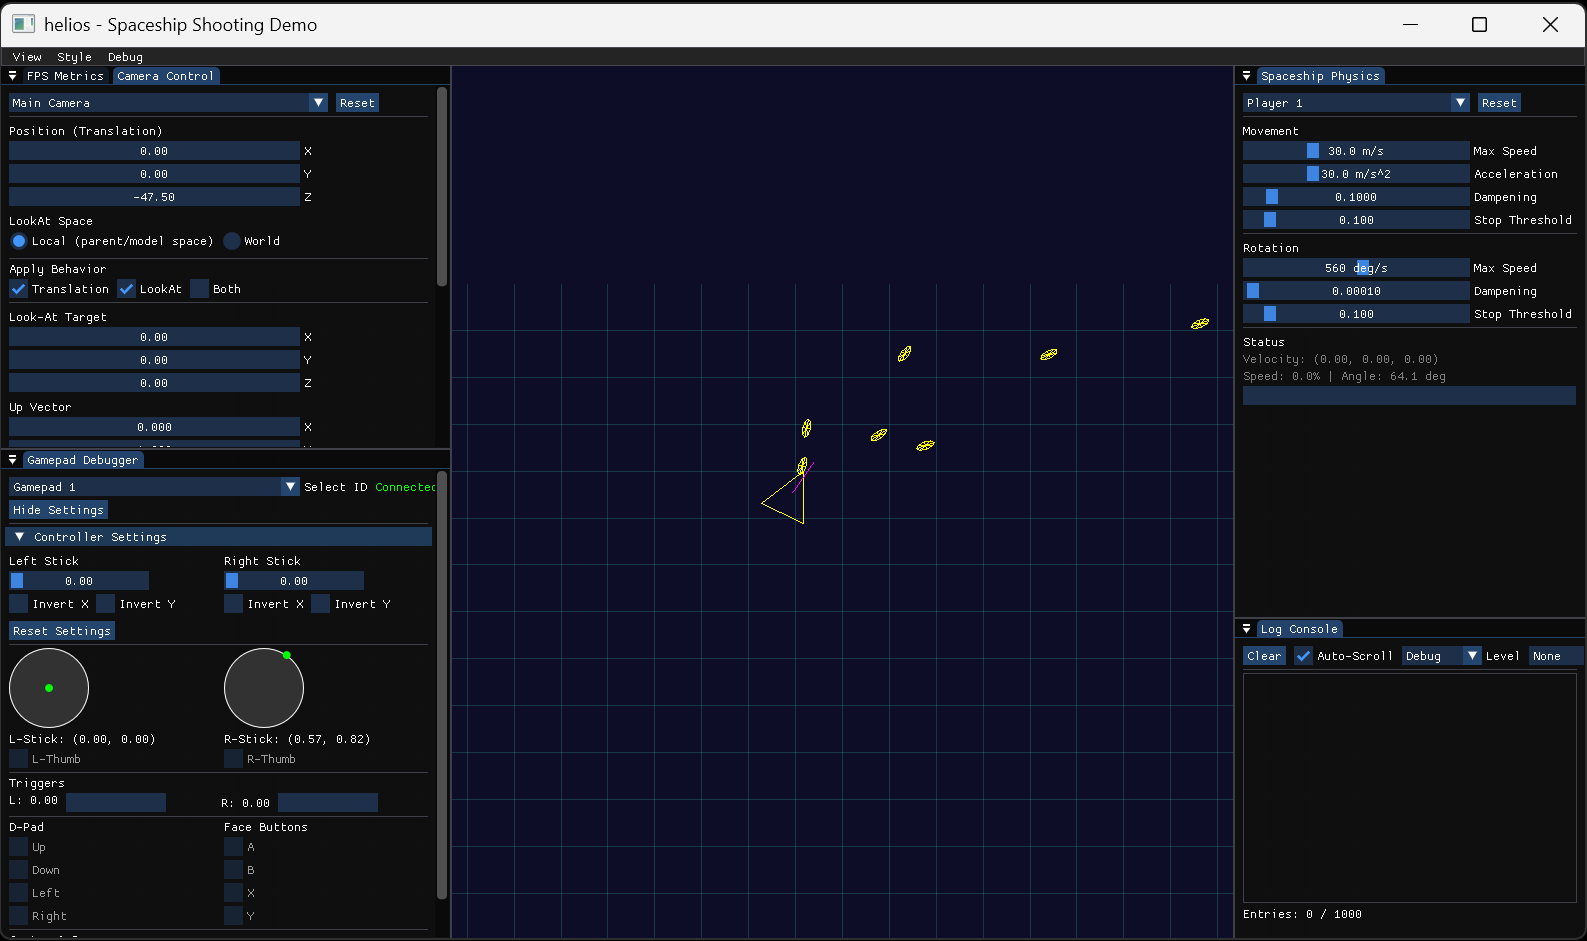
\includegraphics[width=1\columnwidth]{content/de/iterative evolution/img/spaceshipshooting}
    \caption{Screenshot der \textit{Spaceship Shooting Demo} aus Meilenstein 3.
    Die dargestellten Projektile werden über Ellipsen realisiert, die im OpenGL \texttt{GL\_LINE\_LOOP}-Mode gerendert werden. (Quelle: eigene Aufnahme)}
    \label{fig:spaceshipshooting}
\end{figure}


\subsection{Spawn, Despawn und Pooling von Projektilen}

Um die Performance beim Feuern der Projektile zu stabilisieren, wurde ein frühes \textit{Pooling}-Verfahren eingeführt, damit zur Laufzeit keine Heap-Allokationen für die Erstellung neuer Objekte stattfinden müssen (\cite[S. 1074-1079]{Gre24}).
Ein spezialisiertes \texttt{ProjectilePoolSystem} verwaltet dabei die Lebenszyklen der Projektile: Anstatt Objekte bei jedem Schuss neu zu instanziieren und beim Verlassen der Spielwelt zu zerstören, werden despawnte Projektile deaktiviert und für spätere Schussereignisse wiederverwendet.
Dabei prüft das System in jedem Frame, ob die \textit{LevelBounds} noch die

\textit{Axis-Aligned Bounding Box} (im Folgenden \textit{AABB}) eines Projektils beinhalten, und entfernt nötigenfalls das Projektil aus der Spielwelt, um es zurück in den Pool zu legen.\\

Die Logik der \textit{Bounds}-Überprüfung und die Anwendung der gewünschten Reaktion wurde später in das \texttt{LevelBoundsBehavior}-System überführt, das gleichzeitig ein konfigurierbares Verhalten pro \texttt{GameObject} (bzw. \textit{Prefab}) erlaubt, u.,a.: \texttt{Reflect} (mit oder ohne Restitutionskoeffizient), \texttt{Despawn} und \texttt{Stick}.\\

Das Pooling-Konzept wurde in späteren Iterationen der Engine ausgebaut, wofür ein eigenes \textit{Runtime}-System geschaffen wurde (siehe Abschnitt~\ref{sec:runtime_manager}).
Während das initiale Pooling-System Projektile noch als eigenständige \texttt{GameObjects} verwaltet - also $N$ Objekte mit jeweils $M$ Komponenten, deren Zustände auf viele Objektinstanzen verteilt werden -, basiert das spätere Verfahren auf dem \texttt{EntityManager} und \textit{Type-Erased Sparse Sets}.
Hierdurch werden die Daten komponentenweise gebündelt; die Anzahl der in diesem Kontext separat verwalteten Speicherstrukturen reduziert sich damit im Wesentlichen auf die Anzahl der $M$ verschiedenen Komponententypen.
